%"runningheads" enables:
%  - page number on page 2 onwards
%  - title/authors on even/odd pages
%This is good for other readers to enable proper archiving among other papers and pointing to content.
%Even if the title page states the title, when printed and stored in a folder, when blindly opening the folder, one could hit not the title page, but an arbitrary page. Therefore, it is good to have title printed on the pages, too.
\documentclass[a4paper]{llncs}
%\usepackage{algorithm}
%\usepackage[noend]{algpseudocode}
\usepackage[linesnumbered,ruled]{algorithm2e}
\makeatletter
\def\BState{\State\hskip-\ALG@thistlm}
\makeatother
\usepackage{indentfirst}
%Even though `american`, `english` and `USenglish` are synonyms for babel package (according to https://tex.stackexchange.com/questions/12775/babel-english-american-usenglish), the llncs document class is prepared to avoid the overriding of certain names (such as "Abstract." -> "Abstract" or "Fig." -> "Figure") when using `english`, but not when using the other 2.
\usepackage[english]{babel}
\usepackage{amsmath}
\DeclareMathOperator*{\argmin}{arg\,min}

%better font, similar to the default springer font
%cfr-lm is preferred over lmodern. Reasoning at http://tex.stackexchange.com/a/247543/9075
\usepackage[%
rm={oldstyle=false,proportional=true},%
sf={oldstyle=false,proportional=true},%
tt={oldstyle=false,proportional=true,variable=true},%
qt=false%
]{cfr-lm}
%
%if more space is needed, exchange cfr-lm by mathptmx
%\usepackage{mathptmx}

\usepackage{graphicx}

%extended enumerate, such as \begin{compactenum}
\usepackage{paralist}

\usepackage{booktabs}

%put figures inside a text
%\usepackage{picins}
%use
%\piccaptioninside
%\piccaption{...}
%\parpic[r]{\includegraphics ...}
%Text...

%Sorts the citations in the brackets
%\usepackage{cite}

\usepackage[T1]{fontenc}

%for demonstration purposes only
\usepackage[math]{blindtext}

%for easy quotations: \enquote{text}
\usepackage{csquotes}

%enable margin kerning
\usepackage{microtype}

%tweak \url{...}
\usepackage{url}
%nicer // - solution by http://tex.stackexchange.com/a/98470/9075
\makeatletter
\def\Url@twoslashes{\mathchar`\/\@ifnextchar/{\kern-.2em}{}}
\g@addto@macro\UrlSpecials{\do\/{\Url@twoslashes}}
\makeatother
\urlstyle{same}
%improve wrapping of URLs - hint by http://tex.stackexchange.com/a/10419/9075
\makeatletter
\g@addto@macro{\UrlBreaks}{\UrlOrds}
\makeatother
\urldef{\authormail}\path|andy_hm_chung@asiamiles.com|

%diagonal lines in a table - http://tex.stackexchange.com/questions/17745/diagonal-lines-in-table-cell
%slashbox is not available in texlive (due to licensing) and also gives bad results. This, we use diagbox
%\usepackage{diagbox}

%required for pdfcomment later
\usepackage{xcolor}

% new packages BEFORE hyperref
% See also http://tex.stackexchange.com/questions/1863/which-packages-should-be-loaded-after-hyperref-instead-of-before

%enable hyperref without colors and without bookmarks
\usepackage[
%pdfauthor={},
%pdfsubject={},
%pdftitle={},
%pdfkeywords={},
bookmarks=false,
breaklinks=true,
colorlinks=true,
linkcolor=black,
citecolor=black,
urlcolor=black,
%pdfstartpage=19,
pdfpagelayout=SinglePage,
pdfstartview=Fit
]{hyperref}
%enables correct jumping to figures when referencing
\usepackage[all]{hypcap}

%enable nice comments
\usepackage{pdfcomment}
\newcommand{\commentontext}[2]{\colorbox{yellow!60}{#1}\pdfcomment[color={0.234 0.867 0.211},hoffset=-6pt,voffset=10pt,opacity=0.5]{#2}}
\newcommand{\commentatside}[1]{\pdfcomment[color={0.045 0.278 0.643},icon=Note]{#1}}

%compatibality with TODO package
\newcommand{\todo}[1]{\commentatside{#1}}

%enable \cref{...} and \Cref{...} instead of \ref: Type of reference included in the link
\usepackage[capitalise,nameinlink]{cleveref}
%Nice formats for \cref
\crefname{section}{Sect.}{Sect.}
\Crefname{section}{Section}{Sections}

\usepackage{xspace}
%\newcommand{\eg}{e.\,g.\xspace}
%\newcommand{\ie}{i.\,e.\xspace}
\newcommand{\eg}{e.\,g.,\ }
\newcommand{\ie}{i.\,e.,\ }


%introduce \powerset - hint by http://matheplanet.com/matheplanet/nuke/html/viewtopic.php?topic=136492&post_id=997377
\DeclareFontFamily{U}{MnSymbolC}{}
\DeclareSymbolFont{MnSyC}{U}{MnSymbolC}{m}{n}
\DeclareFontShape{U}{MnSymbolC}{m}{n}{
    <-6>  MnSymbolC5
   <6-7>  MnSymbolC6
   <7-8>  MnSymbolC7
   <8-9>  MnSymbolC8
   <9-10> MnSymbolC9
  <10-12> MnSymbolC10
  <12->   MnSymbolC12%
}{}
\DeclareMathSymbol{\powerset}{\mathord}{MnSyC}{180}


% correct bad hyphenation here
\hyphenation{op-tical net-works semi-conduc-tor}

\begin{document}

%Works on MiKTeX only
%hint by http://goemonx.blogspot.de/2012/01/pdflatex-ligaturen-und-copynpaste.html
%also http://tex.stackexchange.com/questions/4397/make-ligatures-in-linux-libertine-copyable-and-searchable
%This allows a copy'n'paste of the text from the paper
\input glyphtounicode.tex
\pdfgentounicode=1

\title{ECML/PKDD 2016 Discovery Challenge \\ Bank Branch Visits and Customer Acquisition Prediction using Gradient Boosted Trees}
%If Title is too long, use \titlerunning
%\titlerunning{Short Title}

%Single insitute
\author{
    Andy H.M. Chung
}


%If there are too many authors, use \authorrunning
%\authorrunning{First Author et al.}
\institute{
    Data Scientist, Cathay Pacific - Asia Miles
    \\ \authormail
}
\maketitle

\begin{abstract}
We apply gradient boosted trees algorithm for branch visits prediction and credit card acquisition,
 based on customer information and card payment records for the past 2 years along with geolocation information,
 provided by OTP Bank Hungary. In this paper, we describe the algorithms and techniques used.
\end{abstract}

\keywords{Machine Learning, Customer Acquisition, Recommender System}

%%%%%%%%%%%%%%%%%%%%%%%%%%%%%%%%%%%%%%%%%%%%%%%%%%%%%%%%%%%%%%%%%%%%%%%%%%%%%%%
\section{Introduction}
%%%%%%%%%%%%%%%%%%%%%%%%%%%%%%%%%%%%%%%%%%%%%%%%%%%%%%%%%%%%%%%%%%%%%%%%%%%%%%%
Our dataset contains 3 types of information:

\begin{enumerate}
\item Customer transaction time series
\item Customer information (Age, gender, address, income group, etc.)
\item All bank branches geolocation
\end{enumerate}

The training data is a random sample of customers, with transaction records in 2014.
 The testing data is another random sample of customers, with transaction records in the first half of 2015.
 The bank branch visits record and the date at which they registered for a credit card have been removed from the testing data.

We considered two supervised learning tasks:

\begin{enumerate}
    \item Predict the bank branches visited by the customer
    \item Predict the likelihood to apply for a credit card for each customer
\end{enumerate}

For task 1, we predicted top 5 out of 323 branches most likely to be visited $(p_1{}_i, p_2{}_i, ..., p_5{}_i)$ by customer $i$ in the second half of 2015.
The evaluation metric is based on $cosine@5$ for all $N$ customers, defined by
\begin{equation}
cosine@5 = \frac{1}{N} \sum_{i=1}^{N} \frac{\sum_{k=1}^{5} v(p_k{}_i)\hat{v}(p_k{}_i)}{\sqrt{\sum_{k=1}^{5} v(p_k{}_i)^2} \sqrt{\sum_{k=1}^{5} \hat{v}(p_k{}_i)^2}}
\end{equation}
where the actual and predicted number of visits of the top $k$-th branch by customer $i$ is denoted by $v(p_k{}_i)$ and $\hat{v}(p_k{}_i)$ respectively.

For task 2, we predicted the probability to apply for a credit card in the second half of 2015 for each customer.
 The evaluation metric is based on Area Under the Curve ($AUC$).


%%%%%%%%%%%%%%%%%%%%%%%%%%%%%%%%%%%%%%%%%%%%%%%%%%%%%%%%%%%%%%%%%%%%%%%%%%%%%%%
\section{Algorithm}
%%%%%%%%%%%%%%%%%%%%%%%%%%%%%%%%%%%%%%%%%%%%%%%%%%%%%%%%%%%%%%%%%%%%%%%%%%%%%%%
Among many machine learning algorithms, gradient boosted trees proved to have state-of-the-art performance. Based on the existing
 open source packages, we chose XGboost \cite{xgboost} as our algorithm implementation since it is computationally fast.

We will briefly review the algorithm of decision tree and gradient boosted trees.

\subsection{Decision tree}
For a decision tree $y=f(x)$ with $J$ number of leaves,
 it partitions the input space into $J$ disjoint regions $R_1, R_2, ..., R_j$ and modeled as

\begin{equation}
f_m(x) = \sum_{j = 1}^J c_{jm} I(x \in R_{jm})
\end{equation}
where $m$ equals to 1, $I$ is the indicator function and the optimal choice of $\hat c_j{}_m$ is

\begin{equation}
\hat{c}_{jm} = \frac{1}{\lvert R_{jm} \lvert} \sum_{y_i \in R_{jm}} y_i
\end{equation}
where $\lvert R_{jm} \lvert$ is the total number of observations in the region $R_{jm}$.

A greedy approach for an optimal partition is determined at each split by enumerating all the features and possible split points
 and choosing the one such that the loss function $L$ reduction is maximized.

\subsection{Gradient boosted trees}
A gradient boosted trees $F_m(x)$ is updated as follows for every new tree $f_m$ built at iteration $m$:

\begin{equation}
F_m(x) =
\begin{cases}
    f_1(x)                                 & \text{if } m = 1\\
    F_{m-1}(x) + s \gamma_m f_m(x)         & \text{otherwise}
\end{cases}
\end{equation}
where $s$ is the shrinkage parameter and $\gamma_{m}$ is determined by

\begin{equation}
\gamma_m = \argmin_\gamma \sum_{i} L(y_i, F_{m-1}(x_i) + s \gamma f_m(x_i)).
\end{equation}


%%%%%%%%%%%%%%%%%%%%%%%%%%%%%%%%%%%%%%%%%%%%%%%%%%%%%%%%%%%%%%%%%%%%%%%%%%%%%%%
\section{Data Munging and Feature Engineering}
%%%%%%%%%%%%%%%%%%%%%%%%%%%%%%%%%%%%%%%%%%%%%%%%%%%%%%%%%%%%%%%%%%%%%%%%%%%%%%%
For task 1, we used 2014 1st half as training data and 2014 2nd half branch visits as target.
 For each customer there are 323 rows, each row represents whether the customer visited particular branch based on extracted Customer Features,
 Transaction Features and Branch Features.

For task 2, we merged two different time frames into one dataset:

\begin{enumerate}
\item 2014 1st half features, 2014 2nd half credit card registration as target

\item 2014 2nd half features, 2015 1st half credit card registration as target
\end{enumerate}

For each time frame, the customer id is unique. We predicted the target using extracted Customer Features and Transaction Features.

\subsection{Customer Features}
All categorical data such as age group, gender, income group are one-hot-encoded. Address latitude and longitude are treated as continuous variables.

\subsection{Transaction Features}
The transaction time series is broken down monthly. For each month we calculated frequency of different events (high spending, morning transaction, etc.).
 For in-person events with geolocation information, we first calculated the distance using Euclidean distance between the customer address and the events,
 then we calculated the aggregate sum, standard deviation, median, maximum value of the distance grouped by customer and month.

\subsection{Branch Features}
Branch location latitude and longitude are treated as continuous variables. Derived features include popularity of the branch,
 distance between the branch and the customer. Branch index is not used for training.

%%%%%%%%%%%%%%%%%%%%%%%%%%%%%%%%%%%%%%%%%%%%%%%%%%%%%%%%%%%%%%%%%%%%%%%%%%%%%%%
\section{Stacked Generalization}
%%%%%%%%%%%%%%%%%%%%%%%%%%%%%%%%%%%%%%%%%%%%%%%%%%%%%%%%%%%%%%%%%%%%%%%%%%%%%%%
The idea of Stacked Generalization \cite{stacking} is to use a group of first stage models to do prediction,
 followed by a second stage model using all the predictions from first stage models as input features.


For a N-folds stacking:

\begin{enumerate}
 \item Split the training set in $N$ parts: $training_1, training_2, ..., training_N$ using stratified or random split

 \item Predict $testing$ and $training_1$ using original features from $N-1$ folds ($training_2$, $training_3$, $...$, $training_N$) with first stage models

 \item Similarly for $training_2, training_3, ... training_N$, the prediction for testing is the average of $N$ predictions of $testing$

 \item Train the second stage model based on original features and first stage predictions
\end{enumerate}
%



% \begin{algorithm}
%     \SetKwInOut{Input}{Input}
%     \SetKwInOut{Output}{Output}
%
%     \underline{function Stacking} $(df\_train, df\_test, df\_train\_target, num\_folds, stacking\_index,model$)\;
%     \Input{$df\_train$: Dataframe for training features \newline
%            $df\_test$: Dataframe for testing features \newline
%            $df\_train\_target$: Target variable for training data \newline
%            $num\_folds$: number of folds \newline
%            $model$: Prediction Model with method fit and predict
%            }
%     \Output{Stacking Feature}
%
%     \emph{// Randomly split dataset}\\
%
%
%
%
%
%     \For{$k=1$ {\bfseries to} $num\_folds$ }{
%
%         tmp_valid = df_train
%         tmp_train = df_train
%
%
%     }
%
%     \eIf{$b=0$}
%       {
%         return $a$\;
%       }
%       {
%         return Euclid$(b,a\mod b)$\;
%       }
%     \caption{Stacking algorithm}
% \end{algorithm}



We only applied stacking for task 2 but not task 1.
We tried two stacking method separately:
\begin{enumerate}
 \item 2-folds stacking split by two time frames

 \item Stratified 10-folds stacking after merging two time frames
\end{enumerate}

Since stacking index must be fixed in order to avoid leakage, we can only use either 2-folds or 10-folds stacking.
Although 10-folds is a common choice as it provides minimal information loss, we finally decided using 2-folds for two reasons:
\begin{enumerate}
 \item The training data is a combination data in two different time periods. If folds are split by time,
  stacking feature is built based on information from another time period, which is useful to avoid overfitting.

 \item Both 2-folds and 10-folds stacking gives improvement on $AUC$, but 10-folds stacking shows
  discrepancy in improvement between Cross Validation and 30\% of testing data.
\end{enumerate}

In practice, a diversified combination of stacking features from different algorithms (KNN, RandomForest, SVM, NN, etc.)
will outperform stacking using only one single algorithm.
Since we only used XGboost here, we compensated this by building multiple stacking features using randomized parameters to achieve diversification.


\textbf{Fig. 1} shows the task 2 $AUC$ of 5-folds Cross Validation using same parameters and the $AUC$ of prediction on 30\% of testing data.
 There is a strong correlation in $AUC$ between Cross Validation and 30\% of testing data.
 $AUC$ is improved once stacking is applied and we added more randomized stacking features until there is no improvement.

\begin{figure}[ht!]
\centering
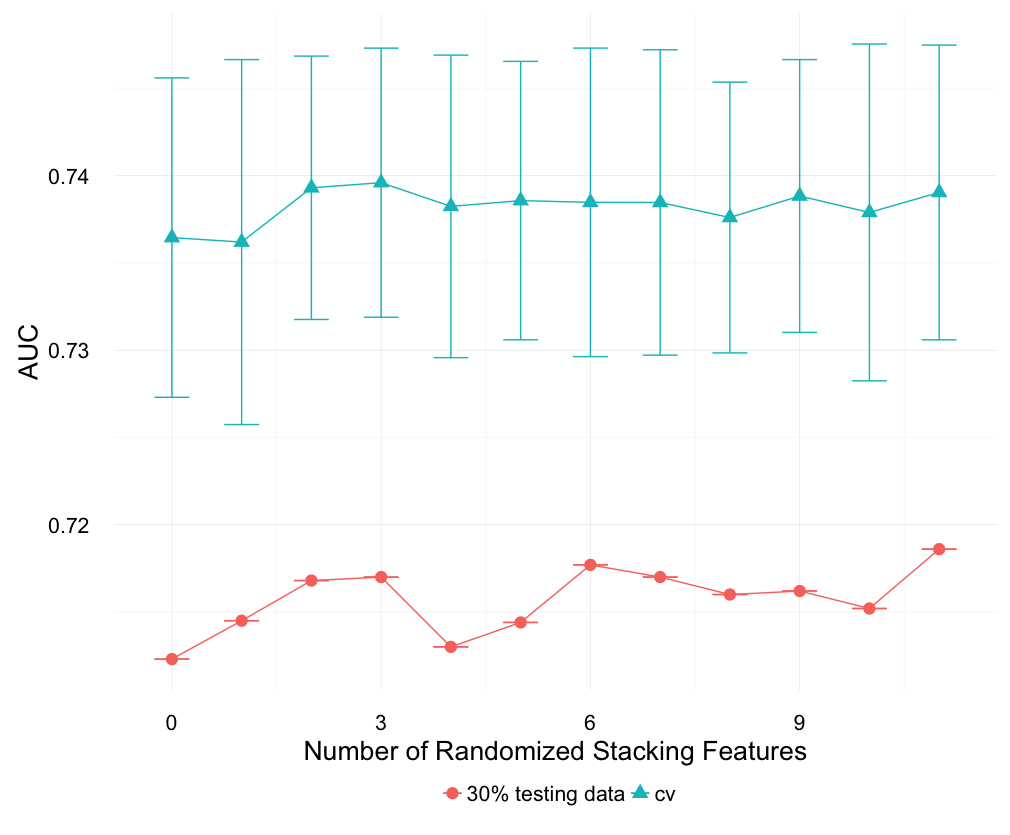
\includegraphics[width=100mm]{Rplot.png}
\caption{Task 2 $AUC$ of 5-folds CV result (Same parameters) and Prediction on 30\% testing data using different number of stacking features.
 The error bar represents one standard deviation of the CV score. \label{overflow}}
\end{figure}




% \begin{algorithm}
% \caption{Stacking}
% \begin{algorithmic}
% \Procedure{MyProcedure}{}
% \State $\textit{stringlen} \gets \text{length of }\textit{string}$
% \State $i \gets \textit{patlen}$
% \BState \emph{top}:
% \If {$i > \textit{stringlen}$} \Return false
% \EndIf
% \State $j \gets \textit{patlen}$
% \BState \emph{loop}:
% \If {$\textit{string}(i) = \textit{path}(j)$}
% \State $j \gets j-1$.
% \State $i \gets i-1$.
% \State \textbf{goto} \emph{loop}.
% \State \textbf{close};
% \EndIf
% \State $i \gets i+\max(\textit{delta}_1(\textit{string}(i)),\textit{delta}_2(j))$.
% \State \textbf{goto} \emph{top}.
% \EndProcedure
% \end{algorithmic}
% \end{algorithm}


%reference
%http://mlwave.com/kaggle-ensembling-guide/
%https://www.researchgate.net/publication/222467943_Stacked_Generalization

%%%%%%%%%%%%%%%%%%%%%%%%%%%%%%%%%%%%%%%%%%%%%%%%%%%%%%%%%%%%%%%%%%%%%%%%%%%%%%%
\section{Hyperparameters Optimization}
%%%%%%%%%%%%%%%%%%%%%%%%%%%%%%%%%%%%%%%%%%%%%%%%%%%%%%%%%%%%%%%%%%%%%%%%%%%%%%%
We applied grid search on a subset of parameters. In general, $max\_depth$, $min\_child\_weight$, $gamma$, $lambda$ and $alpha$ are tuned for model complexity,
 $subsample$, $colsample\_bytree$ are tuned to avoid overfitting, $scale\_pos\_weight$ is used to re-balance dataset.
 In order to speed things up we used a high $eta$ (shrinkage) in the beginning and ranked parameter combinations based on Cross Validation.
 For the parameter combinations with top 5\% ranking, we re-trained the model using a lower $eta$ and selected the one with best Cross Validation result.

For stacking features we used random parameters without optimization
 because in practice stacking perform better when the underlying models are diversified.

\textbf{Table 1} shows the parameters we used during training:

\begin{table}[h!]
  \centering
  \caption{Parameters Optimization for XGboost}
  \label{tab:table1}
  \begin{tabular}{p{3cm}p{4.5cm}p{4cm}p{1cm}}
    \toprule
    Parameters & Description & Grid Search Values & Final Choice \\
    \midrule
    $eta$ & Shrinkage & [0.005, 0.01, 0.05, 0.1] & 0.005 \\
    $max\_depth$ & Maximum depth of trees & [3, 4, 5, 6, 7, 8] & 3 \\
    $colsample\_bytree$ & Subsample ratio of columns when constructing each tree & [0.8, 0.85, 0.9, 0.95, 1] & 0.9 \\
    $colsample\_bylevel$ & Subsample ratio of columns for each split, in each level & [0.8, 0.85, 0.9, 0.95, 1] & 1 \\
    $subsample$ & Subsample ratio of data when constructing each tree & [0.7, 0.8, 0.9, 1] & 1 \\
    $gamma$ & Minimum loss reduction required to make a further partition & [0, 0.025, 0.05, 0.1, 0.3] & 0 \\
    $min\_child\_weight$ & Minimum sum of instance weight (Hessian) required to make a further partition & [1, 3, 5, 7] & 1 \\
    $lambda$ & L2 regularization & [0.1, 0.5, 1, 5, 10, 20] & 5 \\
    $alpha$ & L1 regularization & [0, 0.1, 0.5, 1, 5, 10] & 0 \\
    \bottomrule
  \end{tabular}
\end{table}


%%%%%%%%%%%%%%%%%%%%%%%%%%%%%%%%%%%%%%%%%%%%%%%%%%%%%%%%%%%%%%%%%%%%%%%%%%%%%%%
\section{Performance and Conclusion}
%%%%%%%%%%%%%%%%%%%%%%%%%%%%%%%%%%%%%%%%%%%%%%%%%%%%%%%%%%%%%%%%%%%%%%%%%%%%%%%
For task 1, we predicted the probability of visiting a particular branch for each customer using $Logarithmic Loss$ as the local evaluation metric.
 We selected top 5 branches with highest probability score. The $cosine@5$ on 30\% of the testing data is $\sim0.65$.

The most important features are:

\begin{enumerate}
 \item Distance between the customer and the branch
 \item Popularity of the branch
 \item Location category of the customer

\end{enumerate}

There is still a margin of improvement for task 1, since we transformed the task as a classification problem.
 We discarded too much information in training as we treated customer visiting a branch multiple times same as a single time.

For task 2, we predicted the probability of acquisition for each customer using $AUC$ as the evaluation metric.
The $AUC$ on 30\% of the testing data is $\sim0.719$.

The most important features are:

\begin{enumerate}
 \item How frequent the customer used debit card in the past 6 months

 \item Whether the customer has a credit card in the last month

 \item The total number of POI visited by the customer in the past 6 months

 \item The income group of the customer belongs to mid range
\end{enumerate}

%%%%%%%%%%%%%%%%%%%%%%%%%%%%%%%%%%%%%%%%%%%%%%%%%%%%%%%%%%%%%%%%%%%%%%%%%%%%%%%
\section{Acknowledgments}
%%%%%%%%%%%%%%%%%%%%%%%%%%%%%%%%%%%%%%%%%%%%%%%%%%%%%%%%%%%%%%%%%%%%%%%%%%%%%%%
We thank European Conference on Machine Learning and Principles and Practice of Knowledge Discovery (ECML/PKDD)
and OTP Bank Hungary for hosting the discovery challenge.


%%%%%%%%%%%%%%%%%%%%%%%%%%%%%%%%%%%%%%%%%%%%%%%%%%%%%%%%%%%%%%%%%%%%%%%%%%%%%%%
\bibliographystyle{splncs03}
\bibliography{paper}

%%%%%%%%%%%%%%%%%%%%%%%%%%%%%%%%%%%%%%%%%%%%%%%%%%%%%%%%%%%%%%%%%%%%%%%%%%%%%%%

\end{document}
